\documentclass{article}
\usepackage[italian]{babel}
\usepackage{hyperref}
\usepackage{graphicx}
\graphicspath{ {./imgs/} }

\title{VezGammon - Report finale Team 1 \\ \large Progetto di Ingegneria del Software}
\author{Lorenzo Peronese - Scrum Master}

\begin{document}

\maketitle

\tableofcontents

\newpage

\section{Descrizione del prodotto}
\subsection{Scope}
Per il progetto del corso di Ingegneria del Software, il team ha scelto di lavorare a VezGammon\copyright, un'applicazione web di backgammon. Il progetto ha diversi riferimenti 
alla città di Bologna, in cui è nato e si è sviluppato: in primis ovviamente il nome (\textit{"vez"} viene usato a Bologna come intercalare e significa amico, fratello); 
inoltre una volta nel sito il cursore diventa un simpatico tortellino e la board utilizza i colori rosso e blu, rappresentativi della città. \par
L'applicazione offre un'esperienza di gioco completa con diverse modalità: gli utenti possono sfidarsi in partite locali sullo stesso dispositivo, mettere alla prova 
le proprie abilità contro intelligenze artificiali di vari livelli di difficoltà e confrontarsi online con altri giocatori attraverso un sistema di matchmaking 
o mediante link di invito diretti. È inoltre possibile organizzare tornei a quattro partecipanti, combinando liberamente giocatori reali e agenti intelligenti. \par
Il sistema di classificazione si basa sul metodo Elo, ampiamente utilizzato negli scacchi. Ogni nuovo account parte da una base di 800 punti, che vengono poi 
aggiornati dopo ogni partita online o torneo. Il calcolo dell'aggiornamento tiene conto di diversi fattori: l'esito della partita, l'utilizzo del dado double 
e il punteggio Elo di entrambi i giocatori. Questo sistema garantisce una competizione equilibrata e permette di mantenere una classifica globale, 
dove ogni giocatore può aspirare a raggiungere le posizioni più alte. \par
VezGammon\copyright \: include anche ricche funzionalità social e di progressione. Gli utenti possono consultare (e condividere sui social) in ogni momento statistiche dettagliate delle proprie partite, 
visualizzare grafici che mostrano l'andamento del proprio Elo nel tempo e analizzare i match recenti. Il sistema premia inoltre i giocatori con speciali badge 
al raggiungimento di specifici obiettivi, come vincere un determinato numero di partite o raggiungere certi livelli di punteggio Elo, aggiungendo un ulteriore 
elemento di coinvolgimento e progressione al gioco.

\subsection{Backlog}
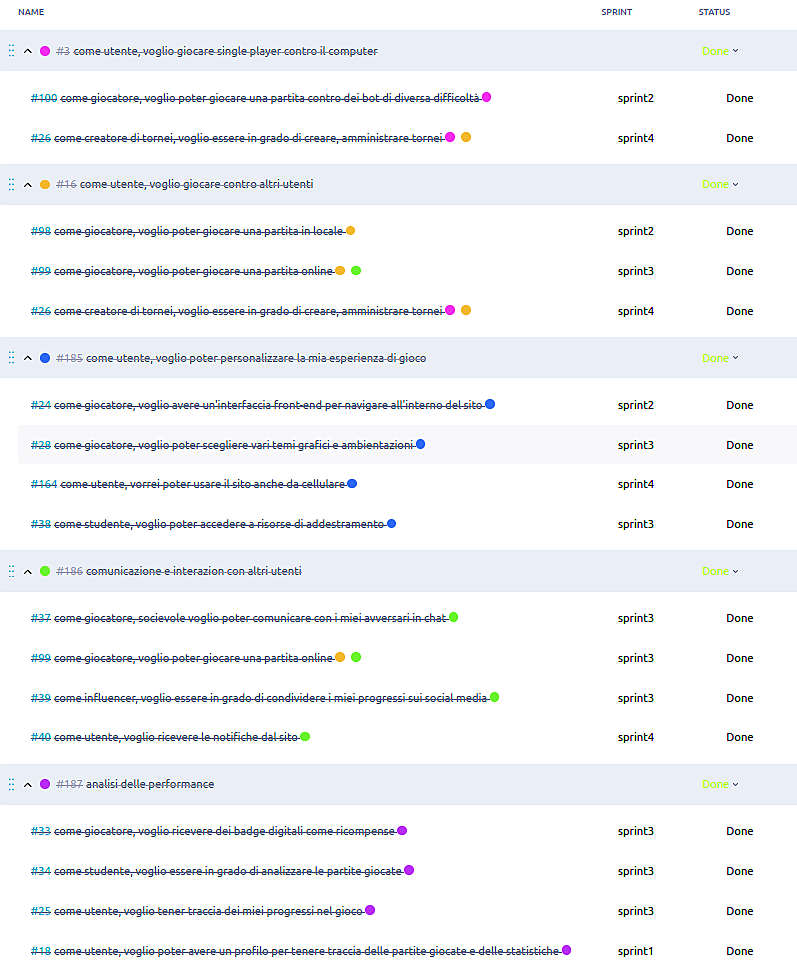
\includegraphics[width=12cm, height=14cm]{backlog}

\subsection{UML}
\subsubsection{Casi d'uso}

\subsubsection{Deployment}

\subsubsection{Classi}

\subsubsection{Tornei}

\section{Sprint 0}

\section{Sprint 1}

\subsection{Goal}

\subsection{Backlog}

\subsection{Incremento}

\subsection{Definition of Done}

\subsection{Esempio di test fatti}

\subsection{Burndown}

\subsection{Retrospettiva}

\section{Sprint 2}

\subsection{Goal}

\subsection{Backlog}

\subsection{Incremento}

\subsection{Definition of Done}

\subsection{Esempio di test fatti}

\subsection{Burndown}

\subsection{Retrospettiva}

\section{Sprint 3}

\subsection{Goal}

\subsection{Backlog}

\subsection{Incremento}

\subsection{Definition of Done}

\subsection{Esempio di test fatti}

\subsection{Burndown}

\subsection{Retrospettiva}

\section{Sprint 4}

\subsection{Goal}

\subsection{Backlog}

\subsection{Incremento}

\subsection{Definition of Done}

\subsection{Esempio di test fatti}

\subsection{Burndown}

\subsection{Retrospettiva}

\section{Release sprint}

\section{Descrizione del processo}

Il team ha deciso di comune accordo e su richiesta del \textit{Product Owner} di dedicare al progetto quattro sprint di due settimane ciascuno, in aggiunta allo sprint 0, dedicato alle attività di teambuilding
e alla familiarizzazione dell'ambiente di sviluppo, e al release sprint, in cui il focus è andato sulla risoluzione dei bug, qualità del codice e stesura di questo report finale.

\subsection{Il team}

\begin{itemize}
    \item \textbf{Product Owner}: Diego Barbieri
    \item \textbf{Scrum Master}: Lorenzo Peronese
    \item \textbf{DevOps}: Samuele Musiani
    \item \textbf{Developer frontend}: Emanuele Argonni
    \item \textbf{Developer backend}: Fabio Murer
    \item \textbf{Developer backend}: Omar Ayache
\end{itemize}

Il team è composto da sei membri ed è la prima volta che lavoriamo tutti insieme su un progetto di questa portata. Sebbene non ci conoscessimo tutti a vicenda inizialmente, 
alcuni di noi avevano già collaborato durante precedenti attività, sia universitarie che non. Durante gli sprint abbiamo avuto modo 
di approfondire la conoscenza reciproca in un contesto diverso dal solito, rafforzando il rapporto e favorendo una collaborazione più efficace. \par
Prima di iniziare lo sprint 0, il team si è riunito di persona per definire i ruoli; questi sono stati rispettati per la maggior parte, ma con un approccio flessibile: 
lo Scrum Master e il Product Owner hanno aiutato nello sviluppo del frontend, mentre il DevOps ha supportato sia il frontend che il backend quando necessario. 
Questa versatilità si è rivelata vincente e ha permesso di ottimizzare il lavoro e affrontare le sfide che si sono presentate in modo più efficace e collaborativo.

\subsection{Teambuilding}

\subsection{Gitinspector}

\subsection{Strumenti di comunicazione}
Per comunicare tra noi abbiamo deciso di usare MatterMost, una piattaforma di chat e condivisione interamente open-source. Come per gli altri servizi, anche MatterMost 
è stato self-hostato sotto il dominio vezgammon.it per avere un maggiore controllo sui dati. Questa scelta ha permesso al team di gestire in autonomia 
l'infrastruttura di comunicazione, evitando dipendenze da servizi esterni e assicurando la personalizzazione dell'ambiente in base alle necessità del progetto. \par
MatterMost è stato utilizzato per la comunicazione quotidiana, la condivisione di aggiornamenti e l'organizzazione degli incontri di persona, che si sono svolti con frequenza. 
Gli incontri hanno avuto luogo presso il laboratorio del gruppo ADMstaff, situato nel seminterrato del Dipartimento di Informatica, in Mura Anteo Zamboni 7. \par
Il laboratorio è diventato il punto di riferimento per il team, che vi si è riunito interi pomeriggi per daily scrum, sessioni di pair programming e discussioni sull'avanzamento 
generale del progetto. Questa modalità di lavoro ha favorito una collaborazione continua e diretta, contribuendo significativamente alla coesione del gruppo e al progresso del progetto.

\subsection{Uso di LLM}

\subsection{Deployment del prodotto}

\subsection{Retrospettiva finale con Essence}

\section{Demo 3 min}
Link qui

\section{Artefatti realizzati}

Per il progetto sono stati realizzati e resi disponibili diversi artefatti, sia di prodotto che di processo. Tutto l'ambiente è stato self-hostato per X motivi TODO 

\subsection{Artefatti di processo}

\subsubsection{GitLab (\href{https://gitlab.vezgammon.it}{\texttt{gitlab.vezgammon.it}})}
GitLab è stato utilizzato per la gestione del codice sorgente e per il versioning. Sono stati utilizzati i tag per denotare il Minimun Value Product di ogni sprint.
Il team ha qui configurato il repository, gestito le merge request e segnalato e risolto le issue.  

\subsubsection{Taiga (\href{https://taiga.vezgammon.it}{\texttt{taiga.vezgammon.it}})}
Taiga è stato scelto per la gestione del project management. È stato utilizzato per tracciare le attività, gestire i backlog, definire le storie utente e 
monitorare lo stato di avanzamento del progetto durante gli sprint.

\subsubsection{MatterMost (\href{https://mattermost.vezgammon.it}{\texttt{mattermost.vezgammon.it}})}
MatterMost è stato utilizzato per la comunicazione interna del team. È stata la piattaforma principale per gli scambi di messaggi, la condivisione di aggiornamenti 
e per accordarsi sugli incontri quotidiani.

\subsubsection{Jenkins (\href{https://jenkins.vezgammon.it}{\texttt{jenkins.vezgammon.it}})}
Jenkins è stato utilizzato per l'automazione del flusso di lavoro tramite CI/CD e dei processi di build e deployment. Il team ha configurato job automatici per 
costruire, testare e distribuire l'applicazione.

\subsubsection{SonarQube (\href{https://sonarqube.vezgammon.it}{\texttt{sonarqube.vezgammon.it}})}
SonarQube è stato utilizzato per l'analisi della qualità del codice. Il team ha configurato SonarQube per eseguire analisi statiche e rilevare eventuali problematiche 
riguardanti la qualità del codice, la copertura dei test e la manutenzione.

\subsubsection{Status (\href{https://status.vezgammon.it}{\texttt{status.vezgammon.it}})}
Il sistema di monitoraggio dei servizi è stato sviluppato per tenere traccia della disponibilità dei vari strumenti utilizzati nel progetto. 
\'E stato inoltre sviluppato un bot Telegram per avvisare tempestivamente il team di eventuali problemi con il server e/o i singoli servizi.

\subsection{Artefatti di prodotto}

Il team ha configurato due server principali per ospitare l'applicazione:
\begin{itemize}
    \item \textbf{Server di produzione}: \href{https://vezgammon.it}{\texttt{vezgammon.it}}
    \item \textbf{Server di sviluppo}: \href{https://dev.vezgammon.it}{\texttt{dev.vezgammon.it}}
\end{itemize}
Il server di produzione è stato utilizzato per la versione stabile, mentre il server di sviluppo è stato dedicato al testing, al debug e alle fasi di sviluppo continuo.

\end{document}